\documentclass{article}
\usepackage{graphicx} % Required for inserting images
\usepackage{amssymb}
\usepackage{bm}
\usepackage{hyperref}
\usepackage{amsmath}
\usepackage{listings}
\usepackage{xcolor}
\usepackage{geometry}
% \usepackage{showframe} % This line can be used to clearly show the new margins %
\newgeometry{vmargin={25mm}, hmargin={25mm,25mm}} 
\hypersetup{
    colorlinks=true,
    linkcolor=blue,
    filecolor=magenta,      
    urlcolor=blue,
    pdftitle={Overleaf Example},
    pdfpagemode=FullScreen,
    }
\usepackage{graphicx}
\graphicspath{ {./images} }

\title{RareSkills - Advanced Solidity}

\author{Meek Msaki (Meek\#6464)}
\date{May 2023}
\begin{document}
\maketitle
Advanced solidity bootcamp with Dominik Teiml. Summary of \href{https://ethereum.github.io/yellowpaper/paper.pdf}{the ethereum yellow paper}.
\section{Chapter 1}
\section{Chapter 2}
\section{Chapter 3}
\begin{itemize}
    \item$\bm{\sigma}$ - (sigma) World state
    \item $\bm{\mu}$ - (mu) Machine state
    \item $\bm{\Upsilon}$ - (upsilon) Ethereum state transition
    \item $C$ - General cost function
    \item $KEC$ - Keccak-256 hash function
    \item $KEC512$ - Keccak512 hash function
    \item $T$ - Ethereum transaction
    \item $\delta$ - (delta) the number of items required on a stack for a given operation
    \item $\textbf{o}$ - the output data of a message call
    \item $\mathbb{N}$ - a set of scalar non-negative numbers e.g. set of integers smaller than $2^{256}$ denoted by $\mathbb{N}_{256}$
    \item $\mathbb{B}$ - a set of byte sequences, e.g. bytes 32 is denoted by $\mathbb{B}_{32}$
    \item $f$ - a function
    \item $\ell$ - a function which evaluates the last item in the given sequence
\end{itemize}

\section{Chapter 4}

\subsection{The World State}
\begin{itemize}
    \item$\bm{\sigma}$ - represents world state or state. It is a \underline{mapping between addresses (160-bit) and account states}, a data structure serialised as Recursive Length Prefix (RLP)
    \begin{itemize}
        \item$\bm{\sigma}$[$a$] = \textbf{Account state} - The state of ethereum accounts has four fields
        \begin{itemize}
            \item$\bm{\sigma}$[$a$]$_n$ = account's  \textbf{nounce state}
            \item$\bm{\sigma}$[$a$]$_b$ = account's \textbf{balance state}
            \item$\bm{\sigma}$[$a$]$_s$ =  256-bit hash \textbf{storageRoot} of merkle patricia trie root node that encodes storage contents (a mapping between 256-bit integer values)
            \begin{itemize}
                \item For Eternally Owned Accounts, $\bm{\sigma}[a]_s = \varnothing$ 
                \item For Contract accounts $\bm{\sigma}[a]_s \neq \varnothing$ 
                \item It's not hash of the merkle trie root but for the key/value pairs stored within $\bm{\sigma}[a]_s \equiv TRIE(L_I^*((\bm{\sigma}[a]_s))$ 
            \end{itemize} 
            \item$\bm{\sigma}[a]_c =$ \textbf{codeHash} -  Keccak 256-bit hash of contract bytecode that gets executed when the account receives a message call
            \begin{itemize}
                \item For Eternally Owned Accounts, $\bm{\sigma}$[$a$]$_c$ = $\varnothing$ 
                \item For contract accounts $\bm{\sigma}[a]_c \neq \varnothing$ 
                
                - $KEC(\textbf{b}) = \bm{\sigma}[a]_c$, \textbf{b} to denote the contract's EVM bytecode
                
            \end{itemize}
        \end{itemize}
        \item An account is \textit{empty} if it has no code $\bm{\sigma}[a]_c = \varnothing$, zero nonce $\bm{\sigma}[a]_n = 0$ and zero balance $\bm{\sigma}[a]_b = 0$
            \begin{itemize}
                \item $EMPTY(\bm{\sigma}, a) \equiv {\bm{\sigma}[a]}_c = {KEC(())} \wedge {\bm{\sigma}[a]}_n = 0 \wedge {\bm{\sigma}[a]}_b = 0$
            \end{itemize}
        \item An account is \textit{dead} if its account state is non-existent or empty 
            \begin{itemize}
                \item $DEAD(\bm{\sigma}, a) \equiv \bm{\sigma}[a] = \varnothing \lor EMPTY(\bm{\sigma}, a)$
            \end{itemize}
    \end{itemize}


\end{itemize}
\subsection{The Transaction}
\begin{itemize}
    \item $T$ - a single cryptographically sigend instruction by an EOA. 
    \item $S$ - maps transaction to the sender with ECDSA SECP-256k1 curve (hash of the transaction excepting three signature fields). 
    \item Assert the sender of a transaction $T$ represents $S(T)$
    \item $L_T(T) \equiv \left\{
            \begin{array}{ll}
                      (T_n, T_p, T_g, T_t, T_v, T_i, T_w, T_r, T_s) \text{ if } T_t = \varnothing \\
                      (T_n, T_p, T_g, T_t, T_v, T_d, T_w, T_r, T_s) \text{ } otherwise \\
                    \end{array}
                  \right.$ - Specifies how to serialize a transaction
    
    \underline{The sender of a transaction cannot be a contract}

    There are two subtype of transactions
    \begin{itemize}
        \item Those that result in message calls
        \item Those that result in creation of new accounts with associated code ('contract creation')
    \end{itemize} 
    
    \underline{EIP-1559: Fee market change (type 2) transactions have:}
    \begin{itemize}
        \item $T_n$ - Transaction nounce for the sender, $T_n \in \mathbb{N}_{256}$
        \item $T_g$ - Gas Price, $T_p \in \mathbb{N}_{256}$
        \item $T_g$ - Gas Limit, $T_g \in \mathbb{N}_{256}$
        \item $T_t$ - To (160-bit address),  $T_t \in \left\{
            \begin{array}{ll}
                      \mathbb{B}_{20} \text{ if } T_t \neq \varnothing \\
                      \mathbb{B}_{0} \text{ contract creation}\\
                    \end{array}
                  \right.
            $
        \item $T_i$ - EVM-code for account initialization, $T_i \in \mathbb{B}$
        \item $T_r, T_s$ - Signature of the transaction used to determine the sender of the transaction
        \item $T_w$ - \textbf{ChainId} and \textbf{yParity} are combined to form single value $T_w = 2\beta + 35 + T_y$ (see EIP-155 by Buterin [2016b]), $T_w \in \mathbb{N}_{256}$
        \item $T_x$ - EIP-2718 transaction type, $T_x \in \{1,2\}$
        \item $T_p$ - Gas Price, $T_p \in \mathbb{N}_{256}$
        \item $T_g$ - Gas Limit, $T_g \in \mathbb{N}_{256}$
        \item $T_v$ - Value, $T_v \in \mathbb{N}_{256}$
        \item $T_r, T_s$ - Signature of the transaction used to determine the sender of the transaction, $T_r \in \mathbb{N}_{256}$, $T_s \in \mathbb{N}_{256}$
        \item $T\bm{_A}$ - Access list (Legacy transactions don't have access list)
        \item $T_c$ - Chain ID, $T_c = \beta$
        \item $T_y$ - yParity signature, $T_y \in \mathbb{N}_{1}$ (bool)
        \item $T_i$ - init is an unlimited size byte array specifying the EVM-code for contract initialization procedure, it is fragment that returns a \textbf{body}, $T_i \in \mathbb{B}$
        \item $T_d$ - data byte array specifying input data of a message call, $T_d \in \mathbb{B}$

    \end{itemize}
    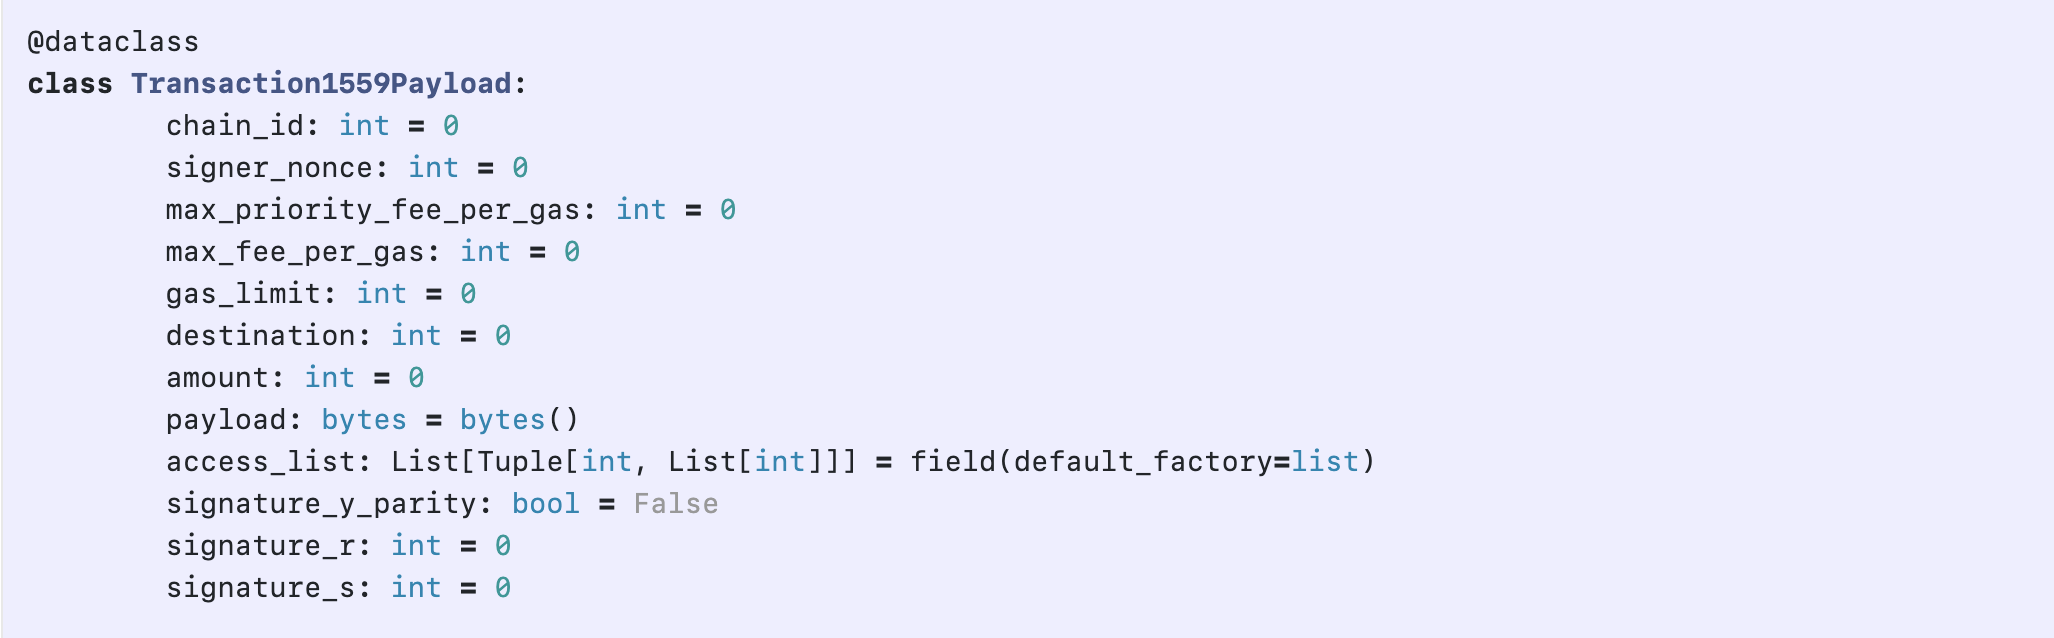
\includegraphics[width=\textwidth]{EIP1559.png}
    
    \underline{EIP-2930 (type 1) transactions also have:}
    \begin{itemize}
        \item $T\bm{_A}$ - Access list (Legacy transactions don't have access list)
         \item $T_c$ - Chain ID must equal chain ID $\beta$, $T_c = \beta$
        \item $T_y$ - yParity signature 
    \end{itemize}
    
    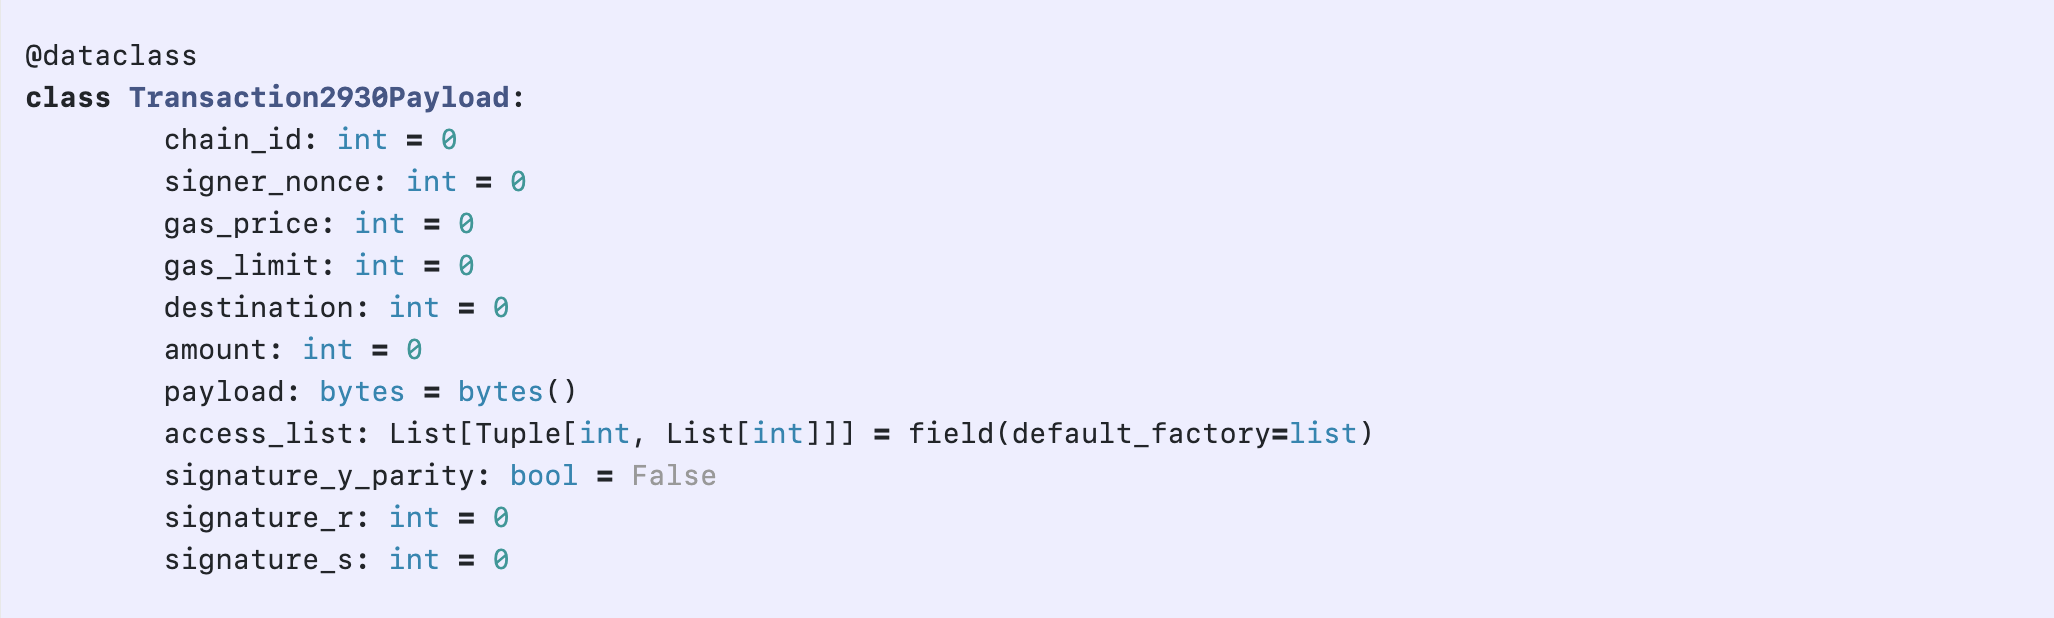
\includegraphics[width=\textwidth]{EIP2930.png}
    
\end{itemize}

\subsection{The Block}

The Block, $B \equiv (B_H, B_T, B_U)$, is a collection of the following relevant pieces  of information: 

\begin{enumerate}
    \item \textbf{T} - information corresponding to \underline{transactions}
    \begin{enumerate}
        \item[$-$] $B_{T}$ - A series of transactions from this block
    \end{enumerate}
    \item \textbf{U} - A set of block headers, ($ommers^2$) or \underline{uncles}
    \begin{enumerate}
        \item[$-$] $B_U$ - A list of ommer block headers
    \end{enumerate}
    \item \textit{H} - represents block \underline{\textit{header}}, which contains: $\mathbb{B} = \{B : B \in \mathbb{B}\lor \| B \| = n\}$
    \begin{enumerate}
        \item $H_p$ - \textbf{parentHash} - keccak256-bit hash of the parent's block header
        \begin{enumerate}
            \item[$-$] $H_p \in \mathbb{B}_{32}$
            \item[$-$] $H_p \equiv KEC(P(B_H))$ where $P(B_H)$ is the parent block header of $B$
            \item[$-$] $TRIE(L_s(\sigma)) = P(B_H)_{H_r}$
        \end{enumerate}
        \item $H_o$ - \textbf{ommersHash} - keccak256-bit hash of the ommers list of this block
        \begin{enumerate}
            \item[$-$] $H_o \in \mathbb{B}_{32}$
            \item[$-$] $H_o \equiv KEC(RLP(L_H^*(B_U)))$
        \end{enumerate}
        \item $H_c$ - \textbf{beneficiary} - 160-bit address that receives of all fees collected from successful mining this block
        \begin{enumerate}
            \item[$-$] $H_c \in \mathbb{B}_{20}$
        \end{enumerate}
        \item $H_r$ - \textbf{stateRoot} - keccak256 hash of the root node of the state trie after all transaction are executed on this block, $H_r \equiv KEC(TRIE(L_s(\Pi(\sigma,B))))$
        \begin{enumerate}
            \item[$-$] $H_r \in \mathbb{B}_{32}$
            \item[$-$] $\Pi$ - transaction state's accummulation function
        \end{enumerate}
        \item $H_t$ - \textbf{transactionRoot} - keccak26-Bit hash of trie's root node with this block's transactions
        \begin{enumerate}
            \item[$-$] $H_t \in \mathbb{B}_{32}$
            \item[$-$] $H_t \equiv KEC(TRIE(\{\forall i < \| B_{\textbf{T}} \|, i \in \mathbb{N} : p_T(i, B_{\textbf{T}}[i])\}))$
        \end{enumerate}
        \item $H_e$ - \textbf{receiptsRoot} - keccak256-bit hash of the trie's root node containing receipt's of each transaction from this block, $H_e \equiv KEC(TRIE(\{\forall i< \|B_R\|, i \in \mathbb{N} :  p_R(i, B_R[i])\}))$
        \begin{enumerate}
            \item[$-$] $H_e \in \mathbb{B}_{32}$
            \item[$-$] $B_R$ - values steming from the computation of transactions, specificaly transaction receipts
        \end{enumerate}
        \item $H_b$ - \textbf{logsBloom} - Bloom filter from indexable info (logger addres and log topics) contained in each log entry from the receipt of each transaction in this block
        \begin{enumerate}
            \item[$-$] $H_b \in \mathbb{B}_{256}$
        \end{enumerate}
        \item $H_d$ - \textbf{difficulty} - a scalar value of the difficulty level of this block
        \begin{enumerate}
            \item[$-$] $H_d \in \mathbb{N}$
        \end{enumerate}
        \item $H_i$ - \textbf{number} - a scalar value equal to the number of ancestor blocks
        \begin{enumerate}
            \item[$-$] $H_i \in \mathbb{N}$
        \end{enumerate}
        \item $H_l$ - \textbf{gasLimit} - a scalar value equal to the current limit of gas expenditure per block
        \begin{enumerate}
            \item[$-$] $H_l \in \mathbb{N}$
        \end{enumerate}
        \item $H_g$ - \textbf{gasUsed} - a scalar value equal to the total gas used in transactions in this block
        \begin{enumerate}
            \item[$-$] $H_g \in \mathbb{N}$
        \end{enumerate}
        \item $H_s$ - \textbf{timestamp} - a scalar value equal to the output of Unix's time() at the block's inception
        \begin{enumerate}
            \item[$-$] $H_s \in \mathbb{N}_{256}$
        \end{enumerate}
        \item $H_x$ - \textbf{extraData} - arbitrary byte array data relevant to this block, must be 32 bytes or less
        \begin{enumerate}
            \item[$-$] $H_x \in \mathbb{B}$
        \end{enumerate}
        \item $H_m$ - \textbf{mixHash} - 256-bit hash which combined with nonce, proves a sufficient amount of computation has been carried out in this block
        \begin{enumerate}
            \item[$-$] $H_m \in \mathbb{B}_{32}$
        \end{enumerate}
        \item $H_n$ - \textbf{nonce} - 64-but value which combined with mix-hash proves sufficient computation has been carried out
        \begin{enumerate}
            \item[$-$] $H_n \in \mathbb{B}_8$
        \end{enumerate}
    \end{enumerate}
\end{enumerate}

\subsubsection{Transaction Receipt}

\begin{itemize}
    \item[$-$] $B_R[i]$ - receipt for the $i^{th}$  transaction in an index-keyed trie who's root is recorded in the header as $H_e$
    \item[$-$] $R  \equiv (R_x, R_z, R_u, R_b, R_l)$
    \item[$-$] $L_R(R) \equiv (R_z, R_u, R_b, R_l)$ - the $L_R$ function prepares tx receipt to be transformed into an RLP-serialized bytes array
    \item $R$ - Transaction receipt (a tuple of 5 items):

    \begin{enumerate}
        \item $R_x$ - equal to the corresponding transaction type
        \item $R_z$ - status code of the transaction, $R_z \in \mathbb{N}$ (non-negative integer)
        \item $R_u$ - cumulative gas used, $R_u \in \mathbb{N}$ (non-negative integer)
        \item $R_l$ - a series of logs entries ($O_0, O_1,...$) created through execution of the transaction:
        \begin{enumerate}
            \item A log entry, $O$, is a tuple of: $O \equiv (O_a, (O_{t0}, O_{t1},...), O_d)$ 
            \begin{enumerate}
                \item $O_a$ - logger's  address,  $O_a \in \mathbb{B}_{20}$ 
                \item $O_t$ - series of 32-byte log topics, $\forall x \in O_t : x \in \mathbb{B}_{32}$
                \item $O_d$ - some number of bytes data, $O_d \in \mathbb{B}$
            \end{enumerate}
        \end{enumerate}
        \item $R_b$ - the Bloom filter composed from the information in the logs, $R_b \in \mathbb{B}_{256}$
        \begin{enumerate}
            \item $M$ - a function (bloom filter) to reduce a log entry into a single 256-byte hash:
            \begin{enumerate}
                \item $M(O) \equiv \bigvee _{x \in {O_a}\cup O_t}(M_{3:2048}(x))$
                \begin{enumerate}
                    \item $M_{3:2048}$ - a specialized Bloom filter that sets three bits out of 2048, given an arbitrary byte sequence
                    \item $M_{3:2048}$ - takes the low-order 11 bits of each of the first 3 pairs of bytes in a keccak-256 hash of the byte sequence
                    \item $M_{3:2048}(\textbf{x} : \textbf{x} \in \mathbb{B})  \equiv \textbf{y} : \textbf{y} \in \mathbb{B}_{256}$ where:
                    \begin{itemize}
                        \item $\textbf{y} = (0,0,0,...,0)$ except:
                        \item $\forall i \in \{0,2,4\} : B_{2047-m(\textbf{x},i)}(\textbf{y}) = 1$
                        \item $B$ - a bit reference function
                    \end{itemize}
                    \item ${m(\textbf{x},i) \equiv KEC(\textbf{x})[i,i+1] \mod 2048}$ 
                \end{enumerate}
            \end{enumerate} 
        \end{enumerate}
    \end{enumerate}
\end{itemize}

\subsubsection{Holistic Validity}

\begin{itemize}
    \item identity of state when transactions executed in order on the base state
    \begin{itemize}
        \item $H_r \equiv TRIE(L_s(\Pi(\sigma,B))) \land$
        \item $H_o \equiv KEC(RLP(L_H^*(B_U))) \land$
        \item $H_t \equiv TRIE(\{\forall i < \| B_{\textbf{T}} \|, i \in \mathbb{N} : p_T(i, B_{\textbf{T}}[i])\}) \land$ 
        \item $H_e \equiv TRIE(\{\forall i< \|B_R\|, i \in \mathbb{N} :  p_R(i, B_R[i])\}) \land$ 
        \item $\bigvee _{r \in B_R}(\textbf{r}_b)$
        
    \end{itemize}
\end{itemize}

\paragraph{(TODO: to be continued... pg 6/41)}

\subsubsection{Serialization}
\begin{itemize}
    \item $L_H(H)$ - preparation function for block header
    \begin{itemize}
        \item $L_H(H) \equiv (H_p, H_o, H_r, H_t, H_e, H_b, H_d, H_i, H_l, H_g, H_s, H_x, H_m, H_n)$
    \end{itemize}
    \item $L_B(B)$ - preparation function for block
    \begin{itemize}
        \item $L_B(B) \equiv (L_H(B_H),\tilde{L}_T^*(B_H), L_H^*(B_U))$
        \item $\tilde{L}_T$ - takes special care of EIP-2718 transactions
    \end{itemize}
\end{itemize}

\subsubsection{Block Header Validity}

\begin{itemize}
    \item[$-$] $P(H) \equiv B' : KEC(RPL(B'_H)) = H_p$ 
    \item[$-$] $H_i \equiv P(H)_{Hi} + 1$ - the block number is the parent's block number uncremented by one 
    \item[$-$] $D(H)$ - canonical difficulty fo a block header $H$ 
    \item[$-$] $\varsigma_{2}$ - $Homestead$ diffuculty parameter
    \item[$-$] $\epsilon$ - exponetial difficulty symbol 
\end{itemize}

\section{Chapter 5}

\section{Chapter 6 (Transaction Execution)}

\begin{itemize}
    \item[$-$] $\Upsilon$ - state transition function
    \item[$-$] $\bm{\sigma}'$ - the post-transactional state 
    \item[$-$] $\bm{\sigma}' = \Upsilon(\sigma, T)$ - $\Upsilon$ is the function, $T$ is the transaction and $\sigma$ the state
    \item[$-$] $\Upsilon^g$ - evaluates amount of gas used in the transaction
    \item[$-$] $\Upsilon^l$ - evaluates transaction's accrued log items
    \item[$-$] $\Upsilon^z$ - evaluates the status code resulting from the transaction
\end{itemize}

\subsection{Substate}

$Accrued \text{ } substate$ ($A$) is the information that is acted upon immediately following the transaction execution

\begin{itemize}
    \item[$-$] $A \equiv (A_s, A_l, A_t, A_r, A_a, A_K)$ - $A$ is a tuple
    \item[$-$] $A_s$ - the self destruct set, a set of accounts that will be discarded following transaction completion
    \item[$-$] $A_l$ - log series of archived and indexable 'checkpoints' in VM code execution
    \item[$-$] $A_t$ - set of touched accounts, which the empty ones are deleted at the end of transaction
    \item[$-$] $A_r$ - the refund balance, from SSTORE instruction when contract storage is reset to zero from non-zero
    \item[$-$] $A_a$ - the set of accessed account addresses
    \item[$-$] $A_K$ - a tuple of a 20-byte account address and a 32-byte storage slot (a set of storage keys) 
    \item[$-$] $A^0$ - an empty accrued substate
    \item[$-$] $A^0 \equiv (\varnothing, (), \varnothing, 0, \pi, \varnothing)$, where: $\pi$ is a set of precompiled addresses
    \item[$-$] $\pi$ - a set of all precompiled addresses 
\end{itemize}

\subsection{Execution}

\begin{itemize}
    \item[$-$] $g_0$ - amount of gas this transaction requires to be paid prior to execution
    % \item[$-$] 
    % \item[$-$] 
    % \item[$-$] 
    % \item[$-$] 
    % \item[$-$] 
\end{itemize}

\end{document}
